% LaTeX template for a short report (written for MSES scenario modelling)
% uses LaTeX documentclass "article" for use of sections (not chapter) and References (not Bibliography)
% for Chapters and Bibliography use "documentclass "report
\documentclass[10pt]{article}   % Use article class with 10pt letter
%\documentclass[10pt]{report}
\usepackage[utf8]{inputenc}

%\usepackage[T1]{fontenc}  % 8-bit encoding, helps hyphenation of accented characters -
% https://tex.stackexchange.com/a/677/42066

% Use A4 paper and set margins:
%\usepackage[a4paper, twoside, top=2.0cm, left=3.0cm, bottom=2.0cm, right=2.0cm]{geometry}
\usepackage[a4paper, twoside, top=2.0cm, left=2.0cm, bottom=2.0cm, right=2.0cm]{geometry}
%\usepackage[a4paper, top=2.5cm, left=2.5cm, bottom=2.5cm, right=2.5cm]{geometry}

\usepackage[english]{babel}  % Hyphenation and more for English

\usepackage{pgf}      % Include graphics inside figures using \pgfimage
\usepackage[font=small, labelfont=bf]{caption}  % Stylize figure, table, etc. captions

\usepackage{parskip}         % Replace paragraph indentations with white lines
\usepackage[hyphens]{url}    % Take care of urls, e.g. wrapping in the Bibliography (hyphens: also break at -)

\usepackage{xspace}   % \xspace saves the user from having to type \  or {} after a macro name in text.

% Use the appendix package for nicer appendices:
%\usepackage[toc,page]{appendix}  % MvdS
\usepackage[titletoc]{appendix}
%\usepackage[toc,page,title]{appendix}  % Use \begin{appendices} ... \end{} iso \appendix

% \usepackage[numbib,numindex]{tocbibind}  % Add ToC, List of Figures/Tables/Code listings, Bibliography and Index to ToC
% \usepackage[]{tocbibind}       % Add ToC, List of Figures/Tables/Code listings, Bibliography and Index to ToC
\usepackage[nottoc]{tocbibind}   % ToC without extra "Contents" entry...

\usepackage{amsmath,amssymb,bbm}
\usepackage{enumerate}         % Choose alternative numberings, e.g. \begin{enumerate}[a.]

\usepackage{listings}          % Code listings
\usepackage[section, above, below]{placeins}  % \FloatBarrier - flush floats before \section by default
% \usepackage{pgf}               % Figures

\usepackage{color}
\definecolor{lightgrey}{rgb}{0.9,0.9,0.9}
\definecolor{darkgreen}{rgb}{0.0,0.6,0.0}

% Citations:

% option1: use natbib/bibtex with MvdS_number_url.bst
%\usepackage[numbers, square]{natbib}  % Use numbered citations with square brackets
%\bibliographystyle{MvdS_number_url}  % Use [1], print url = field  (plain doesn't print urls)

%option2: use biblatex/biber without *.bst file
\usepackage[backend=biber, style=numeric, citestyle=numeric-comp, sorting=none]{biblatex} 
\setlength\bibitemsep{0.5\baselineskip}
\usepackage{csquotes}

% \bibliography{mybibliography} % old-style for backward comp. in preamble for biblatex/bibtex
\addbibresource{mybibliography.bib}  % new syntax for BibLaTeX


\usepackage{fancybox}  % Use \ovalbox for key strokes

\newcommand{\ldf}{\usefont{OT1}{cmr}{m}{n}}     % Select default LaTeX font - Computer Modern Roman
%\newcommand{\ldf}{\usefont{OT1}{cmss}{m}{n}}     % Select default LaTeX font - Computer Modern Sans
%\newcommand{\ldf}{\usefont{OT1}{phv}{m}{n}}     % Select default LaTeX font - Helvetica
\newcommand{\ttbf}{\usefont{OT1}{lmtt}{bx}{n}}  % Select bold typewriter font

%\usepackage[font=sf]{caption}  % Use sans-serif font for float captions - not exactly Helvetica



\newcommand{\note}[1]{\color{red}\textbf{#1}\color{black}\xspace}
\newcommand{\marc}[1]{\color{red}\textbf{Marc: #1}\color{black}\xspace}

\newcommand{\myChapter}[1]{
  \chapter{#1}
  \minitoc  % Create a ToC of this chapter
}


% General expressions:
\newcommand{\eg}{\emph{e.g.}\xspace}
\newcommand{\ie}{\emph{i.e.}\xspace}
\newcommand{\etc}{\emph{et cetera}\xspace}
\newcommand{\ff}{\emph{ff}\xspace}

% CLI symbols:
\newcommand{\pipe}{$|$}      % Needed to avoid | in \index{}
\newcommand{\logor}{$|\,|$}  % Needed to avoid | in \index{}
\newcommand{\home}{\url{~}}  % Home directory


% Often used code names:
\newcommand{\NULL}{\code{NULL}}
\newcommand{\void}{\code{void}}
\newcommand{\stdout}{\code{stdout}}
\newcommand{\stderr}{\code{stderr}}

% Man pages:
\newcommand{\man}[2]{\texttt{man #1 #2}\xspace}
\newcommand{\mancmd}[1]{\texttt{man #1}\xspace}

% Code:
\newcommand{\prototype}[3]{\hspace*{2em}\texttt{#1} {\ttbf #2\ldf}(\texttt{#3});\xspace}  % function prototype
\newcommand{\var}[2]{\hspace*{2em}\texttt{#1} {\ttbf #2\ldf};\xspace}  % variable declaration
\newcommand{\code}[1]{\texttt{#1}\xspace}  % inline code
\newcommand{\codeb}[1]{\ttbf #1\ldf\xspace}  % inline bold code
\newcommand{\codeline}[1]{\hspace*{2em}\texttt{#1}}  % separate code line

\newcommand{\cli}[1]{\noindent\hspace*{2em}\code{\$ #1}}  % command line input
\newcommand{\clir}[1]{\noindent\hspace*{2em}\code{\# #1}}  % command line input root
\newcommand{\clo}[1]{\noindent\hspace*{2em}\code{#1}}  % command line output
\newcommand{\clitem}[1]{\item[\code{\$}] \code{#1}}  % cli in itemized list, with $ as bullet
\newcommand{\clitemb}[1]{\item[\codeb{\$}] \codeb{#1}}  % cli in itemized list, with $ as bullet - bold

\newcommand{\key}[1]{\Ovalbox{\texttt{#1}}\xspace}  % key press/combination
\newcommand{\keyb}[1]{\Ovalbox{\ttbf #1\ldf}\xspace}  % key press/combination bold


% Heat pumps
\newcommand{\COP}{\mathrm{COP}}  % COP in "math mode"
\newcommand{\COPh}{\COP_{\mathrm{heating}}}  % COP_heating in "math mode"

\newcommand{\Qh}{Q_{\mathrm{H}}}
\newcommand{\Qc}{Q_{\mathrm{C}}}
\newcommand{\Th}{T_{\mathrm{H}}}
\newcommand{\Tc}{T_{\mathrm{C}}}

\newcommand{\Tin}{T_{\mathrm{in}}}
\newcommand{\Tout}{T_{\mathrm{out}}}

\newcommand{\Ph}{P_{\mathrm{heat}}}
\newcommand{\Pheat}{P_{\mathrm{heat}}}
\newcommand{\Pc}{P_{\mathrm{cool}}}
\newcommand{\Pcool}{P_{\mathrm{cool}}}
\newcommand{\Pel}{P_{\mathrm{el}}}

\newcommand{\degr}{^\circ}
\newcommand{\tdeg}{$\degr$\xspace}
\newcommand{\degC}{\degr\mathrm{C}}
\newcommand{\tdegC}{$\degC$\xspace}

  % Custom commands

\usepackage[pdftex]{hyperref}
\hypersetup{
  colorlinks = true,  % They get a red box around them if false, better set colour to black?
  linkcolor = blue,
  filecolor = magenta,
  citecolor = blue,
  urlcolor = blue,
  % linkcolor = black,
  % citecolor = black,
  % urlcolor = black,
  pdftitle = House Model References,
  pdfauthor = Trung Nguyen,
  pdfsubject = House Models,
  pdfkeywords = house - models - Python,
  pdfcreator = TeXStudio pdfLaTeX2 on Windows,
  pdfproducer = TeXStudio pdfLaTeX2 on Windows,
  bookmarksnumbered = true,  % Number sections in PDF toc
}

\usepackage[onehalfspacing]{setspace}
\usepackage{float}

\usepackage{graphicx}
\usepackage{multirow}

%\renewcommand{\thesection}{\arabic{section}}  % needed for documentclass "report" with sections

\usepackage{subcaption}


%Document title, author and date (empty)
\title{OSEM}
\author{Paul J.M. van Kan\\
HAN University of Applied Sciences\\
Arnhem, The Netherlands}
% \date{}

\begin{document}
	
\ldf  % Set LaTeX default font

% Set up code listing style:
\lstset{
	language=Python,
	% Fonts:
	basicstyle=\ttfamily\footnotesize,
	%keywordstyle=\ttfamily,
	%identifierstyle=,
	%commentstyle=\ttfamily\scriptsize,
	% B/W code:
	% commentstyle=\ttfamily\itshape,  % Italic
	% stringstyle=\ttfamily,
	% identifierstyle=\ttbf,           % Bold typewriter type
	% keywordstyle=\ttbf,              % Bold tt
	% Colour:
	commentstyle=\scriptsize\ttfamily\color{brown},
	stringstyle=\ttfamily\color{darkgreen},
	identifierstyle=\color{blue},
	keywordstyle=\ttfamily\color{red},
	% Spaces:
	showstringspaces=false,
	breaklines=true,
	breakatwhitespace=true,
	% Line numbering:
	numbers=left,
	numberstyle=\tiny,
	stepnumber=2, 
	numbersep=5pt,
	% Frames:
	frame=single,
	frameround=tttt,
	backgroundcolor=\color{lightgrey},
	morekeywords={pthread_create},
}
%\renewcommand{\thelstlisting}{\thechapter.\arabic{lstlisting}}  % This is the default?
%\numberwithin{lstlisting}{section}  % AMSmath: number code listings per section
%\numberwithin{lstlisting}{chapter}  % AMSmath: number code listings per chapter

\ldf

\maketitle

%\begin{center}
%	\today
%\end{center}

\tableofcontents

\newpage

\section{Introduction}

This document presents the basic information for calculating a house model based on an RC network. 
This category of house models, analogous to electrical impedance networks, may have different numbers of R and C components, and may have various component topologies. 
For the specific model properties, references will be given.


\section{Heat pump model}

In heat transfer theory the basic thermal circuit contains thermal resistances. Heat transfer occurs via conduction, convection and radiation. In analogy with Ohm's Law for electricity, expressions can be derived for the heat transfer rate (analogous to electrical current) and the thermal resistances (analogous to ohmic resistances) in these three modes of heat transfer. The temperature difference plays a role analogous to the electrical voltage difference. These expressions are shown in Fig. \ref{fig:hpsimulink}.
\begin{figure}[H]
	\centering
	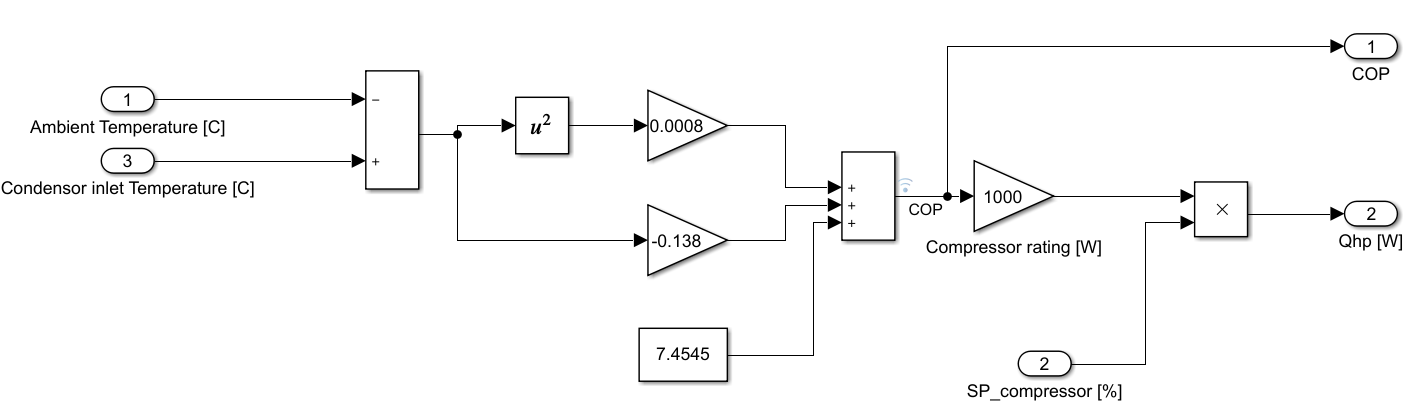
\includegraphics[width=0.8\columnwidth]{Pictures/Heat_Pump.png}
	\caption[Short title]{Heat pump model in Simulink \cite{GIGO}}.
	\label{fig:hpsimulink}
\end{figure}

\lstinputlisting[label=hplist,caption={Heat pump model in Python}, language=Python, linerange={84-88}]{listings/heat_pump.txt}


\begin{figure}[H]
	\centering
	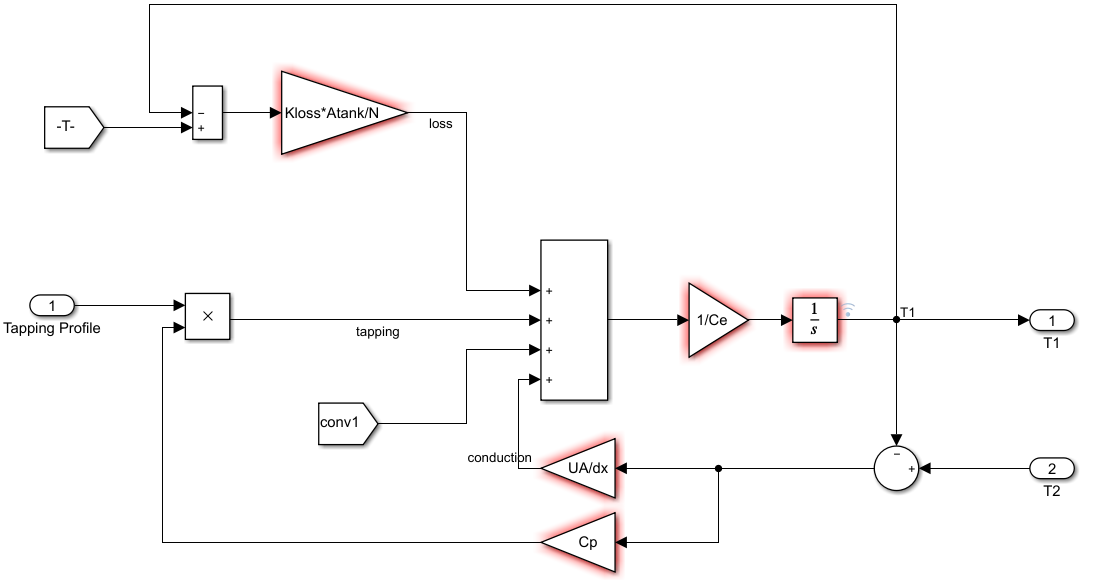
\includegraphics[width=0.8\columnwidth]{Pictures/Layer.png}
	\caption[Short title]{Storage tank layer model in Simulink}.
	\label{fig:layersimulink}
\end{figure}

\begin{figure}[H]
	\centering
	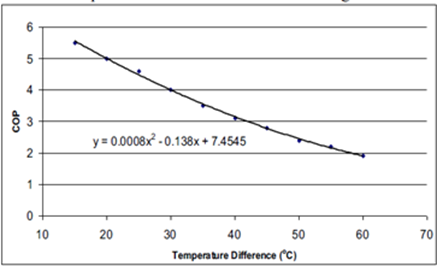
\includegraphics[width=0.8\columnwidth]{Pictures/COPvsDeltaT_Heatpump.png}
	\caption[Short title]{COP vs. Temperature difference between evaporator and condensor side \cite{GIGO}}.
	\label{fig:cop_deltaT}
\end{figure}

Heat transfer rate $\dot{Q}$ in $[W]$

\begin{eqnarray}
	c_{evap} \cdot \frac{dT_{a, out}}{dt} = \dot{m}_{air} \cdot c_{p, air} (T_{a, in} - T_{a, out}) - \dot{Q}_{evap}
\end{eqnarray}

Where $C_{evap} [J/K]$ is the heat capacity of the evaporator. $T_{a,in}$ and $T_{a, out} [K]$ are the temperatures of the air entering and leaving the evaporator, respectively. $\dot{m}_{air} \, [kg/s]$ is the mass flow rate of the air through the evaporator. $\dot{Q}_{evap} [W]$ is the rate of thermal energy delivered by the evaporator.  Note  that  the  last  term $\dot{Q}_{evap}$  can be rewritten as:

\begin{equation}
	\dot{Q}_{evap} = P_{hp} \cdot (COP -1)
\end{equation}

Similarly, from the figure above, the heat balance of the condenser can be written as:

\begin{eqnarray}
	c_{cond} \cdot \frac{dT_{w, out}}{dt} = \dot{m}_{w} \cdot c_{p, w} (T_{w, in} - T_{w, out}) - P_{hp} \cdot COP
\end{eqnarray}

The set of equations presented above characterize the heat delivered by the heat pump as a function of the ambient temperature and the compressor power.

%\newpage


\section{Storage tank model}

The heat balance equation for one layer of the tank can be written as:

\begin{eqnarray}
	c_{layer} \cdot \frac{dT_{layer}}{dt} = \dot{Q}_{conduction} + \dot{Q}_{convection} + \dot{Q}_{tapwater} + \dot{Q}_{heating} + \dot{Q}_{heatloss}
\end{eqnarray}

\subsection{Conduction}

Thermal Law: 
\begin{eqnarray}
	\dot{q} = - \lambda \cdot \frac{T_2 - T_1}{\Delta x} \\
    \text{Heat flux } \dot q  \text{ in } \, [W \cdot m^{-2}] \\
    \lambda \text{ in } [\frac{ W \cdot m}{m^{-2}\cdot K}] 
    = [\frac{W}{m \cdot K}]
\end{eqnarray}	

Thermal conductivity is a material property.


Conduction is the heat transfer between adjacent layers in the tank. This can be elaborated for layer 1 as:

\begin{eqnarray}
	\dot{Q}_1 = (\lambda_{water}\cdot A_{tank} + \lambda_{wall} \cdot A_{wall} )\cdot \frac{T_2 - T_1}{\Delta x}
\end{eqnarray}

Where $(\lambda_{water} \cdot A_{tank} ) / \Delta x$ is the thermal conductance through the interface with layer 2 in $[Wm/K]$. $\Delta x$ is the length (height) of the layer $[m]$.  For the layers 2 to 4: 

\begin{eqnarray}
	\dot{Q}_n = (\lambda_{w}\cdot A_{tank} + \lambda_{wall} \cdot A_{wall}) \cdot \frac{T_{n-1} - 2T_n + T_{n+1}}{\Delta x}
\end{eqnarray}

And finally, for layer 5:

\begin{eqnarray}
	\dot{Q}_5 = (\lambda_{water}\cdot A_{tank} + \lambda_{wall} \cdot A_{wall}) \cdot \frac{T_4 - T_5}{\Delta x}
\end{eqnarray} 

\newpage

\section{Setting up Raspberry Pi}

A Raspberry Pi 4B was received from Contecto. This RPi contains a 16GB SD card with a standard RPi Debian image. Contecto tweaked the settings of the WiFi module, so that it forms an ad-hoc Wifi network with the TinyPico device.

\subsection{Formation of the ad-hoc Wifi network between RPi and TinyPico}

...to be written

\subsection{Getting started with the RPi}

The RPi as delivered is connected to:
\begin{itemize}
	\item a computer screen with the included mini-HDMI to HDMI cable
	\item a USB keyboard
	\item a USB mouse
	\item a 230 V mains outlet socket. Use the included wall adapter with a USB-C interface to the RPi. 
\end{itemize} 

Keep the order of connecting things given above. The RPi will start up immediately upon connecting to the mains voltage.

The RPi comes with the standard device name: \textsf{raspberrypi}, the standard username \textsf{pi} and password-less logging in with complete (sudo) privileges. This is the easiest, but also the most unsafe way of operating a Linux system. Let's do something about it.

Under the Raspberry menu (default location: in the top left corner of the screen) go to \textsf{Preferences $\rightarrow$ Raspberry Pi Configuration}, and open the configuration program.

\begin{itemize}
	\item on the \textsf{System} tab:
	\begin{itemize}
		\item change the hostname to: \textsf{osempi}
		\item disable the auto-login
		\item disable the splash screen
		\item Change Password to \textsf{\#Controller123}
	\end{itemize}
	\item on the \textsf{Interfaces} tab:
		\begin{itemize}
		\item enable SSH
		\item enable VNC
	\end{itemize}
    \item Reboot (on prompt) and login as user \textsf{pi} with your new password
\end{itemize}

Then, a Linux operating system needs some maintenance. Open a \textit{Terminal}. \textsf{RPi Menu $\rightarrow$ Accessories $\rightarrow$ Terminal}. Regularly, the following commands have to be carried out in this terminal window:
\begin{itemize}
	\item \textsf{sudo apt update}
	\item \textsf{sudo apt upgrade}
\end{itemize}

These commands keep the Linux OS fresh and tidy. The \textsf{sudo} in front of the command shows that user \textsf{pi} wants to do an operation that needs system administrator privileges. User \textsf{pi} has these privileges by default, on every RPi in the world. That's why changing the password is the least you should do...

\subsection{Building a network with the RPi}

The RPi as delivered has a WiFi interface which is dedicated to the TinyPico device. The consequence is that the RPi has to connected to your home network with a RJ-45 ethernet cable. The IP address, given to the RPi by the DHCP server of your modem, can not be predicted, but after connecting the cable it can be found by the command:
\begin{itemize}
	\item \textsf{ifconfig}
	\item find the IP address \emph{e.g.} 192.168.178.30 under \textsf{eth0:}
\end{itemize}

Keep the hostname, username, password and IP address at hand for further use.

\subsection{Connecting the RPi to your PC}

The first time you log in to a new RPi, you have to connect a screen, mouse and keyboard. Once you have enabled the SSH server and VNC server on the RPi, you have three options:

\begin{itemize}
	\item continue with screen, mouse and keyboard
	\item use a VNC client on your PC, which connects remotely to the desktop of the RPi. Go to \url{https://www.realvnc.com/en/connect/download/viewer/}  and download VNC Viewer for Windows (OSX, Linux). Install VNC viewer and make a new connection with your RPi. You need the data kept at hand from the previous paragraph. You get the graphical desktop of the RPi as a window on your PC screen. Your PC mouse and keyboard operate on the RPi desktop as well.
	\item use a terminal connection via SSH. Go to \url{https://www.chiark.greenend.org.uk/~sgtatham/putty/} and download \textsf{putty-64bit-0.xx-installer.msi}. Install it and make a connection to the IP address of your RPi. Note that Putty will provide a RPi Linux Terminal only.
\end{itemize}

\subsection{Connecting to the RPi from Matlab on your PC }

When you have Matlab on your PC,and the right subscription license, there is an option to connect to the RPi from Matlab.  

\begin{itemize}
	\item Go to \url{https://nl.mathworks.com/help/supportpkg/raspberrypiio/ug/install-support-for-raspberry-pi-hardware.html}. The recipe given for installing the \textbf{MATLAB Support Package for Raspberry Pi Hardware} is given there. Do not carry out the setup option, offered during installation.
	\item Check the correct installation in Matlab: Add-Ons $\rightarrow$ Manage Add-Ons.
	\item In a similar way, install and check the installation of the \textbf{Simulink Support Package for Raspberry Pi Hardware}.
\end{itemize}

\begin{figure}[ht]
	\centering
	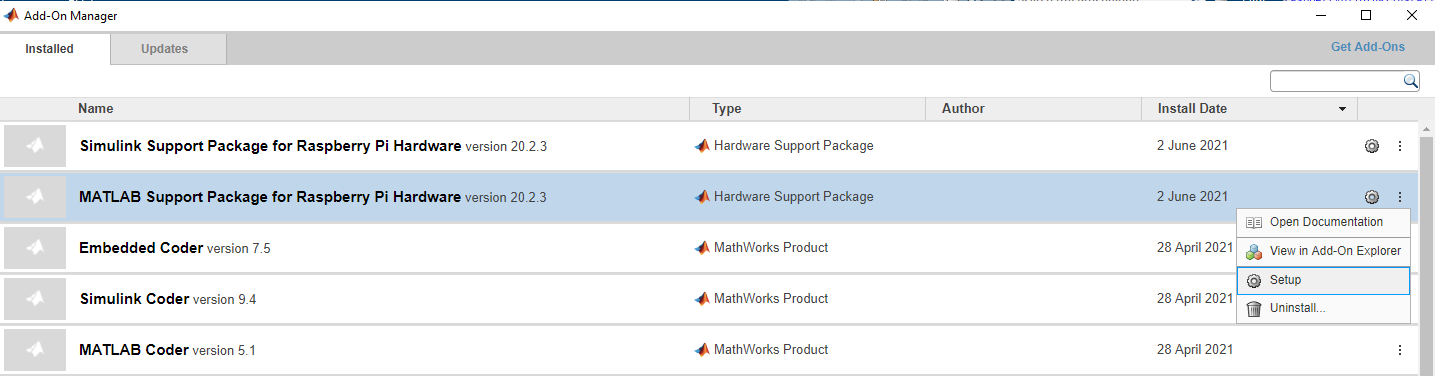
\includegraphics[width=.8\linewidth]{Pictures/Setup RPi.png}  
	\caption{}
	\label{fig:setup}
\end{figure}

\begin{figure}[ht]
	\begin{subfigure}{.3\textwidth}
		\centering
		% include first image
		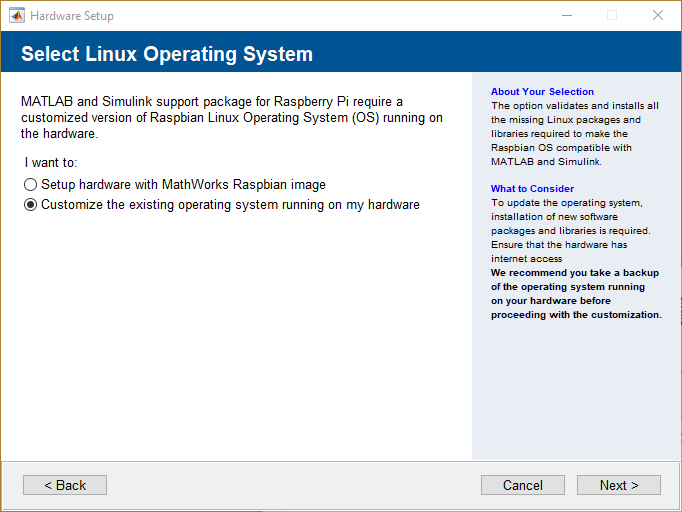
\includegraphics[width=.8\linewidth]{Pictures/Connect RPi 01.png}  
		\caption{}
		\label{fig:sub-first}
	\end{subfigure}
	\begin{subfigure}{.3\textwidth}
		\centering
		% include second image
		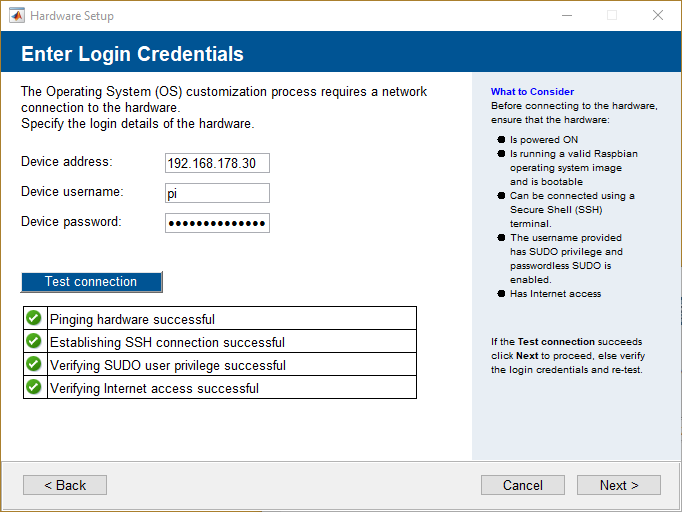
\includegraphics[width=.8\linewidth]{Pictures/Connect RPi 03.png}  
		\caption{}
		\label{fig:sub-second}
	\end{subfigure}
	\begin{subfigure}{.3\textwidth}
		\centering
		% include second image
		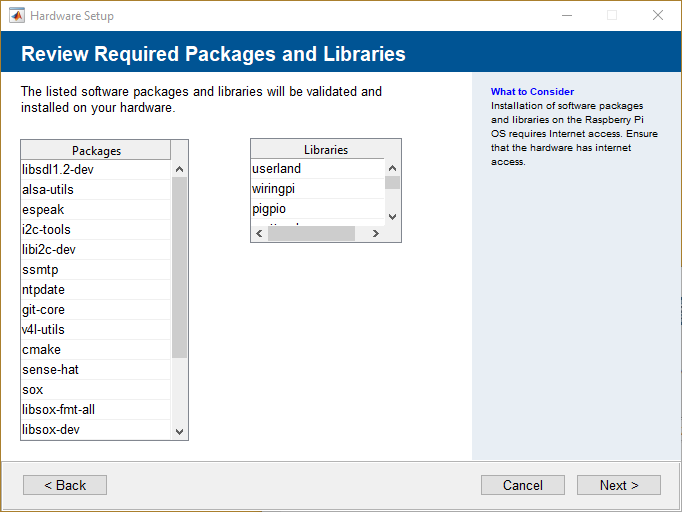
\includegraphics[width=.9\linewidth]{Pictures/Connect RPi 04.png}  
		\caption{}
		\label{fig:sub-third}
	\end{subfigure}
	\newline
	\begin{subfigure}{.3\textwidth}
		\centering
		% include first image
		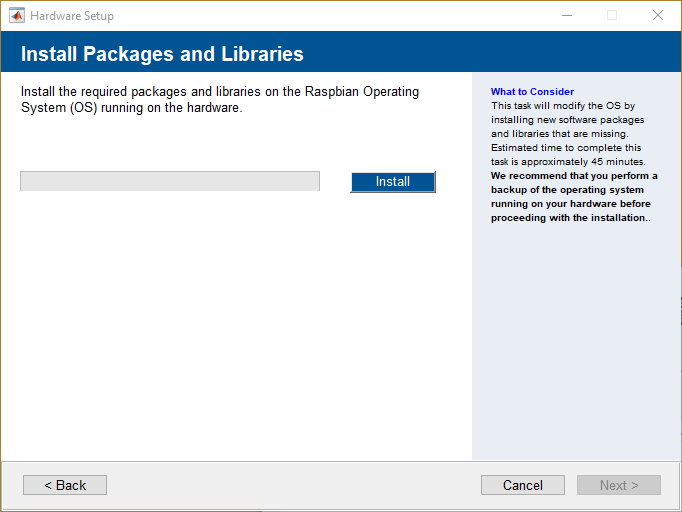
\includegraphics[width=.9\linewidth]{Pictures/Connect RPi 05.png}  
		\caption{}
		\label{fig:sub-fourth}
	\end{subfigure}
	\begin{subfigure}{.3\textwidth}
		\centering
		% include second image
		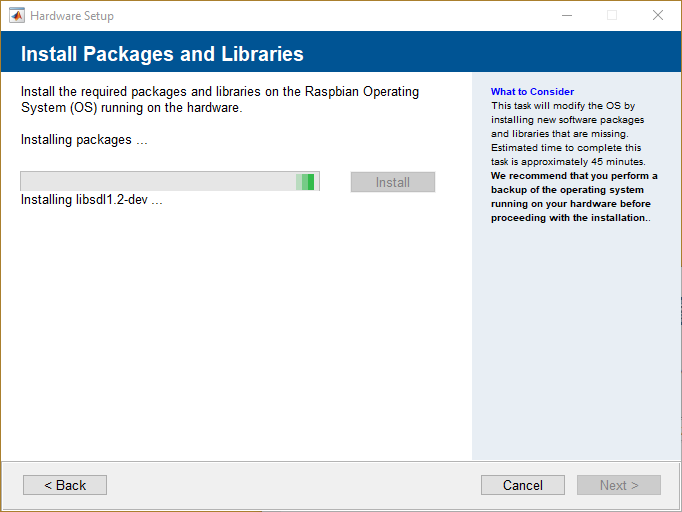
\includegraphics[width=.9\linewidth]{Pictures/Connect RPi 06.png}  
		\caption{}
		\label{fig:sub-fifth}
	\end{subfigure}
	\begin{subfigure}{.3\textwidth}
		\centering
		% include second image
		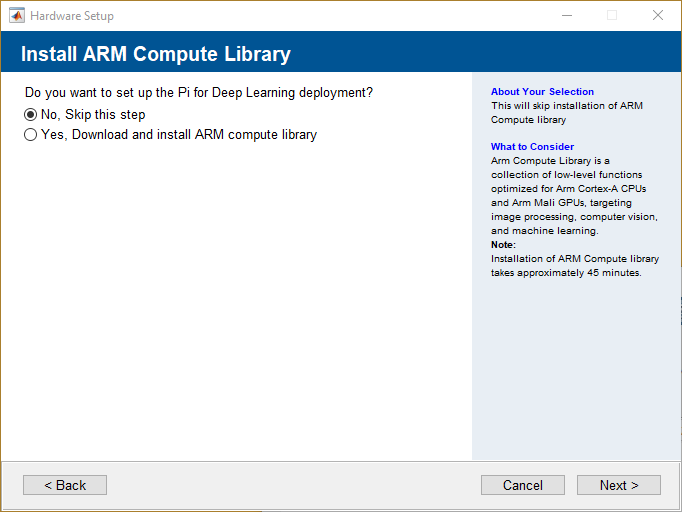
\includegraphics[width=.9\linewidth]{Pictures/Connect RPi 08.png}  
		\caption{}
		\label{fig:sub-sixth}
	\end{subfigure}
	\newline
	\begin{subfigure}{.3\textwidth}
		\centering
		% include second image
		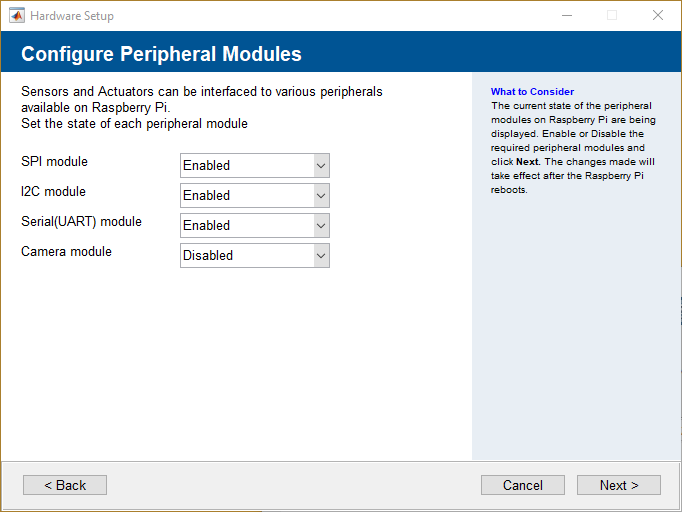
\includegraphics[width=.9\linewidth]{Pictures/Connect RPi 09.png}  
		\caption{}
		\label{fig:sub-seventh}
	\end{subfigure}
	\begin{subfigure}{.3\textwidth}
		\centering
		% include second image
		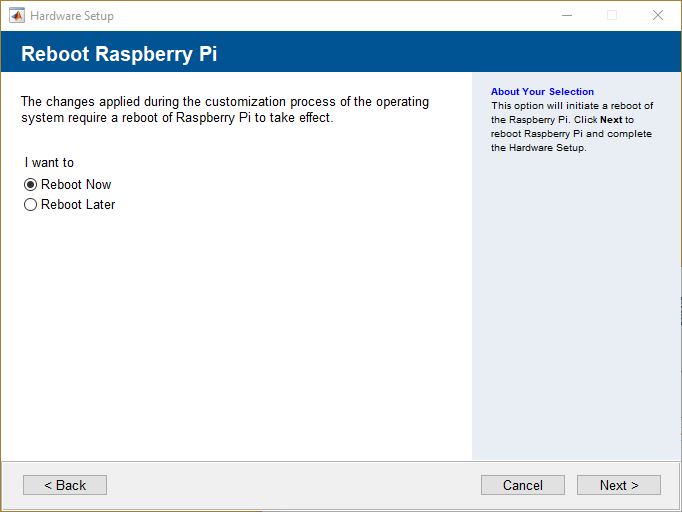
\includegraphics[width=.9\linewidth]{Pictures/Connect RPi 10.png}  
		\caption{}
		\label{fig:sub-eighth}
	\end{subfigure}
	\begin{subfigure}{.3\textwidth}
		\centering
		% include second image
		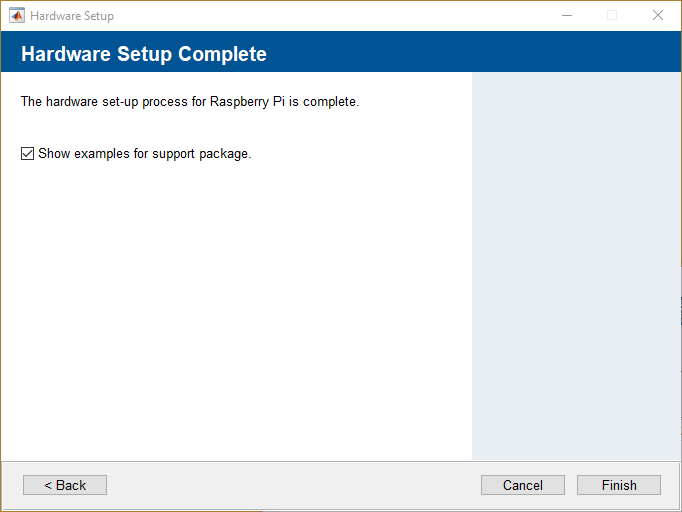
\includegraphics[width=.9\linewidth]{Pictures/Connect RPi 11.png}  
		\caption{}
		\label{fig:sub-ninth}
	\end{subfigure}
	\caption{Setup of connection to Raspberry Pi in Matlab environment}
	\label{fig:fig}
\end{figure}

After the installation of the two Support Packages, keep the Add-On manager Window of Matlab open and click the Settings symbol (cogwheel) of the Matlab Support Package (see Fig. \ref{fig:setup}). In the setup procedure a connection with the RPi is established, and then a number of Linux packages will be installed on the RPi. (see Fig. \ref{fig:fig}) It is important to check "Customize..."in the dialog of Fig. \ref{fig:sub-first}. Then the Matlab softwae is \emph{added} to the SD card of the RPi, and this card is not overwritten, as will happen when the first option in Fig. \ref{fig:sub-first} is chosen.

A similar procedure can be followed for the Simulink Support package. It may be that the setup for both Matlab and Simulink is identical. We will find out if the Simulink setup is necessary or not after the Matlab setup has been carried out already.

See also: \cite{RPi_1, RPi_Connecting, RPi_Getting_Started} \url{https://nl.mathworks.com/videos/install-the-matlab-support-package-for-raspberry-pi-94266.html}

\textbf{Note:} after reboot following the setup dialog of the Support Package, the VNC server seems to be unreachable from the PC.
Disabling the VNC server, reboot of the RPi, re-enabling the VNC server and rebooting the RPi again seems to remedy this Matlab mayhem. The connection on the PC in the VNC client has to be deleted, and a new connection to the RPi has to be created. Then the VNC connection works again.

\subsection{Deployment of Open Source Controller on the Raspberry Pi}

After installation of the Matlab and Simulink Support packages for the Raspberry Pi, a Matlab function can be "translated" into an executable (*.elf) program for the ARM processor of the RPi, downloaded to the RPi and executed (deployed) on the RPi. This can be done from the Windows Matlab environment, as shown in \cite{RPi_2, RPi_Deploying, RPi_Target}:

\url{https://nl.mathworks.com/videos/deploy-matlab-algorithms-on-raspberry-pi-1591965724601.html}

\subsubsection{Converting the OSEM Matlab MPC script into a function}

... to be written

\subsubsection{Deploying the OSEM MPC function on the RPi}

... to be written

\subsubsection{Running the MPC program on the RPi as an executable in the Linux terminal}

...to be written

\subsection{Adding MQTT communication from the RPi to the TinyPico}

... to be written







%\section{2 Zones house model 7R-4C network} 
	
The equivalent electrical 7R-4C network with components and topology is given in Fig. \ref{fig:eq7R4C}.

\begin{figure}[H]
	\centering
	\includegraphics[width=1.0\columnwidth]{Pictures/2_Zones_house_circuits.png}
	\caption[Short title]{R-C circuits of 2 zones house model}
	\label{fig:eq7R4C}
	\end{figure}

with:\\
\begin{itemize}
    \item \texttt{T\_outdoor} : outdoor temperature [$\degr C$] 
    \item \texttt{T\_air\_1}  : zone 1 air temperature [$\degr C$]
    \item \texttt{T\_walls}   : wall temperature [$\degr C$]
    \item \texttt{T\_air\_2}  : zone 2 air temperature [$\degr C$]
    \item \texttt{T\_cc}      : temperature of the concrete layer between zone 1 and zone 2 [$\degr C$]
    \item \texttt{R\_air\_1\_outdoor} : outdoor resistance valus.
    \item \texttt{R\_wall\_1} : walls resistance value.
    \item \texttt{R\_wall\_2} : walls resistance value.
    \item \texttt{R\_cc}      : concrete resistance value.
    \item \texttt{R\_air\_12} : resistance value of air flow from zone 1 to zone 2.
    \item \texttt{R\_air\_21} : resistance value of air flow from zone 2 to zone 1.

\end{itemize}

\newpage

%\section{NEN and ISO}

The list of NEN and ISO standards used in the calculation:

\begin{itemize}
    \item NTA 8800
    \item NEN 1068
    \item ISO 6946
    \item ISO 10077-2
    \item NEN 7120
\end{itemize}

%\newpage

%\bibliography{mybibliography}
\printbibliography[heading=bibintoc]

\end{document}
